%TC:envir minted 1 xall 
%TC:envir algorithmic 1 xall

% Include tables in word count
%TC:envir table 0 word
%TC:envir tabular 1 word

% Include footnotes in word count
%TC:macro \footnote [text]
%TC:macro \footnotetext [text]

%TC:group minted 0 0
%TC:macro \mintinline [ignore]
%TC:macro \colb [ignore]
%TC:macro \hyperref [ignore]

You will need three Raspberry Pis: two acting as hosts and one as the router. You will also need two Ethernet cables and two USB-to-Ethernet adapters. Use the cables to connect both your hosts to the router as shown below. Static router addresses have been defined by the P4 program.

\begin{figure}[htbp]
  \centering
    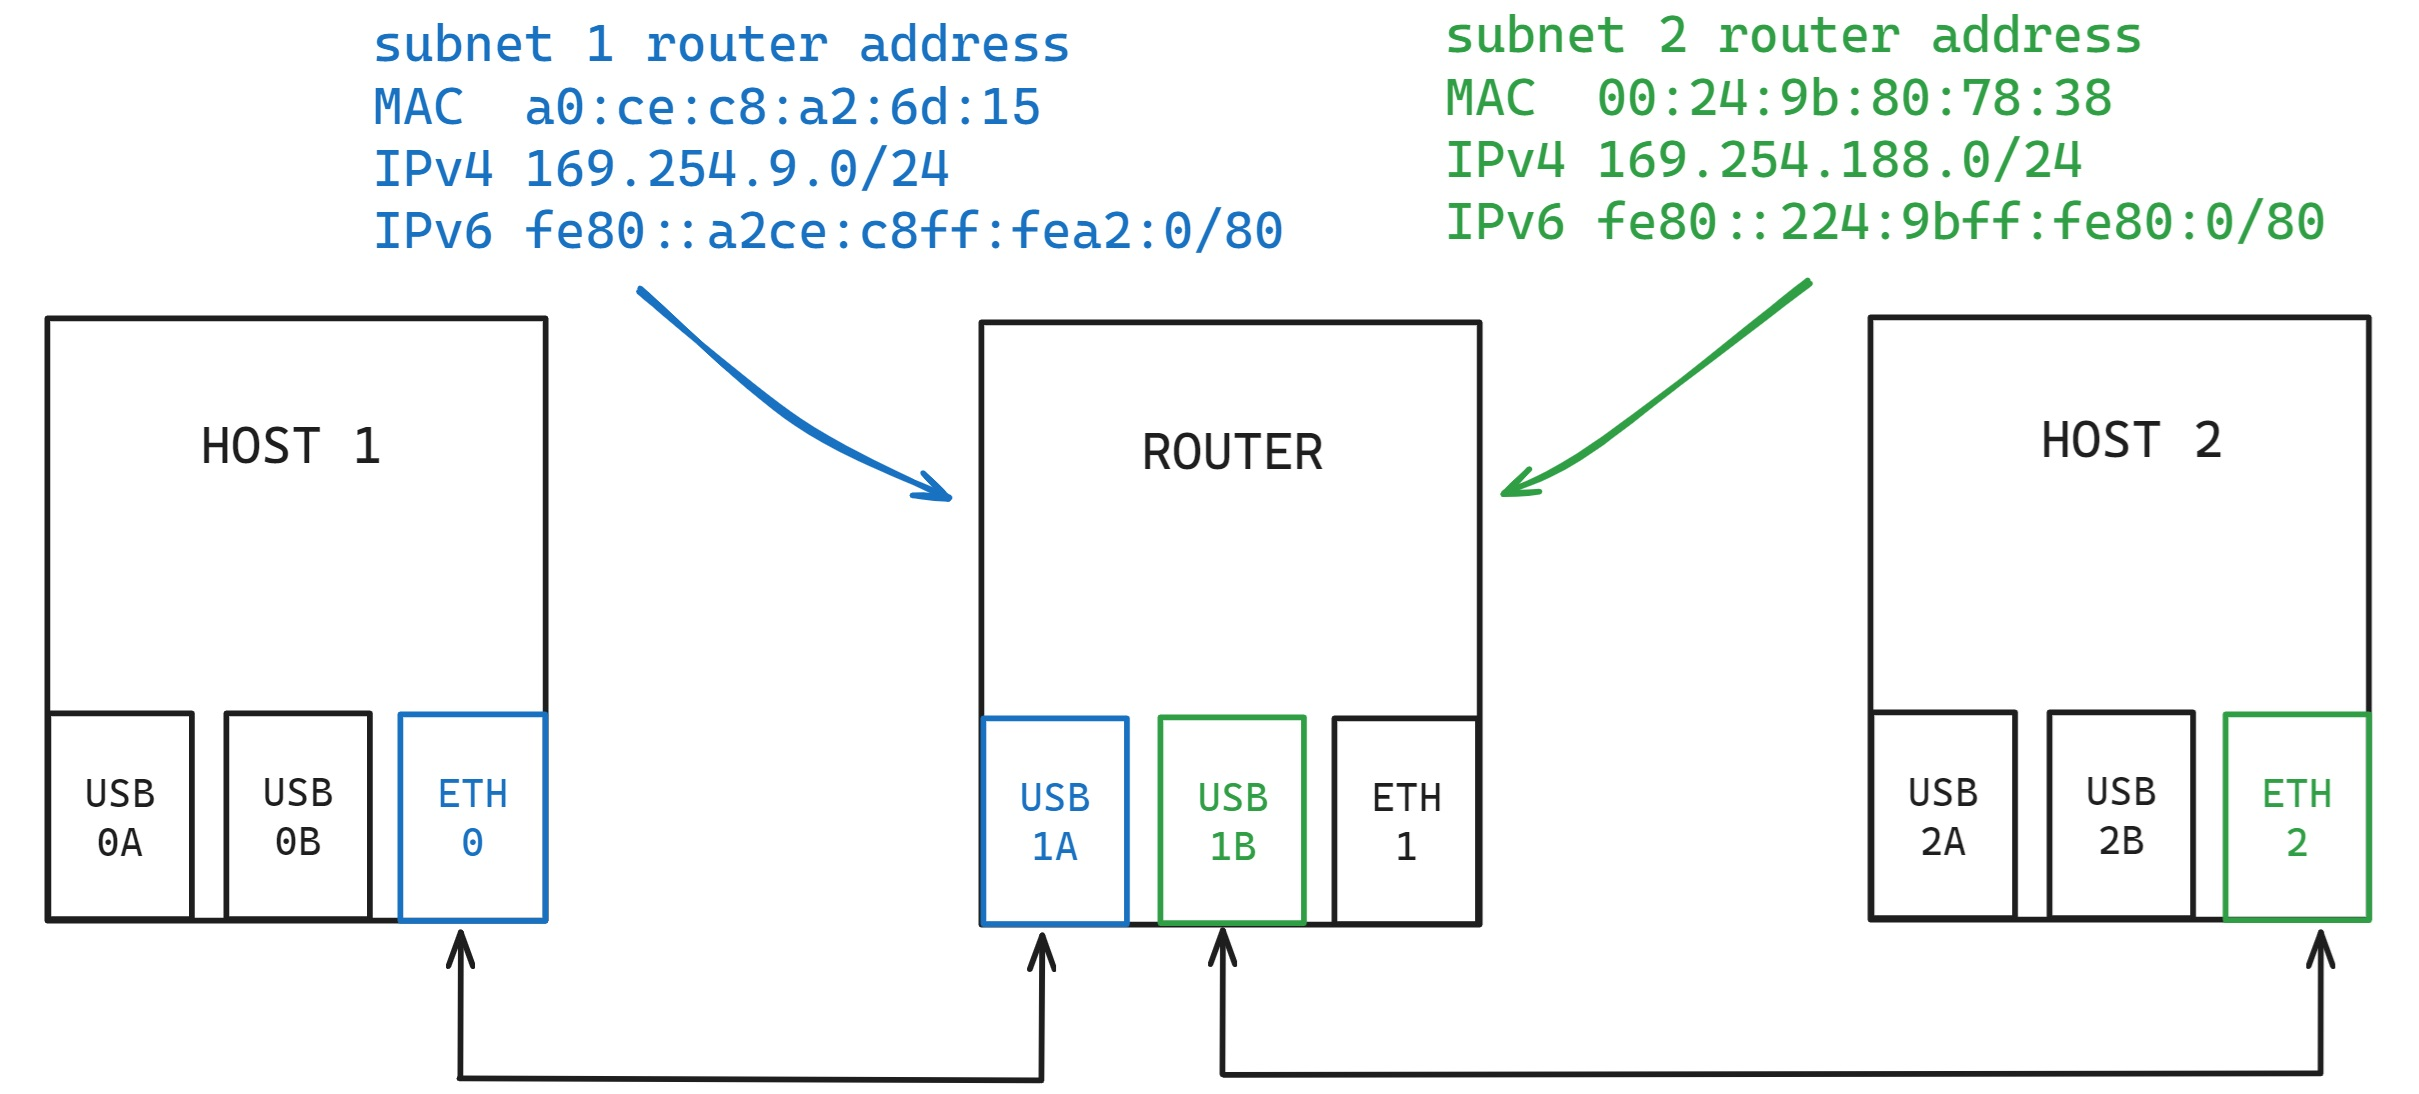
\includegraphics[width=1\textwidth]{figures/appendices/dualstack_setup.jpg}
\end{figure}

Run \texttt{ip a} on the router to learn the MAC and IP addresses of the USB ports connected to your hosts. Edit the P4 program to define constant static router IPv4, IPv6 and MAC addresses (at the top of the program) such that you have one entry for each subnet. These will be referred to as \texttt{IPV4ra}, \texttt{IPV6ra}, \texttt{MACra} and \texttt{IPV4rb}, \texttt{IPV6rb}, \texttt{MACrb}. The MAC addresses should match the router’s port MAC addresses, and the IP addresses should belong to the same subnets as the ports. 

Choose IP addresses \texttt{IPV4a}, \texttt{IPV6a} and \texttt{IPV4b}, \texttt{IPV6b} for the hosts such that they belong to the same subnet as their respective router USB ports. Also run \texttt{ip a} on the hosts to learn their MAC addresses \texttt{MACa} and \texttt{MACb}.

On Host 1, open a command prompt and run the following commands.

To set the host’s IP addresses:
\begin{quote}
    \texttt{sudo ifconfig eth0 IPv4a}
    
    \texttt{sudo ifconfig eth0 inet6 add IPv6a}
\end{quote}

To add routes from Host 1 to the router:
\begin{quote}
    \texttt{sudo ip route add dev eth0 IPv4ra}
    
    \texttt{sudo ip -6 route add dev eth0 IPv6ra}
\end{quote}

To add routes from Host 1 to Host 2:
\begin{quote}
    \texttt{sudo ip route add dev eth0 IPv4b}
    
    \texttt{sudo ip -6 route add dev eth0 IPv6b}
\end{quote}

To check neighbour entry tables (they should initially be empty on port \texttt{eth0}):
\begin{quote}
    \texttt{sudo arp -a}
    
    \texttt{sudo ip -6 neigh show}
\end{quote}

Run the same commands on Host 2, swapping all addresses of Host 1 and Host 2, and using subnet 2’s router address instead of subnet 1’s.

Start the P4 program on the router and, using the CLI (or by using a \texttt{commands.txt} file, as explained in Appendix A), enter the following six commands to populate the IPv4 tables:
\begin{quote}
    \texttt{table\_add MyIngress.ipv4\_lpm MyIngress.forward IPV4a/32 => MACa 0}

    \texttt{table\_add MyIngress.ipv4\_lpm MyIngress.forward IPV4b/32 => MACb 1}
    
    \texttt{table\_add MyIngress.arp\_responder MyIngress.arp\_reply IPV4a => MACa}
    
    \texttt{table\_add MyIngress.arp\_responder MyIngress.arp\_reply IPV4b => MACb}

    \texttt{table\_add MyIngress.arp\_responder MyIngress.arp\_reply IPV4ra => MACra}

    \texttt{table\_add MyIngress.arp\_responder MyIngress.arp\_reply IPV4rb => MACrb}
\end{quote}

And enter the following six commands to populate the IPv6 tables:
\begin{quote}
    \texttt{table\_add MyIngress.ipv6\_lpm MyIngress.forward IPV6a/128 => MACa 0}
    
    \texttt{table\_add MyIngress.ipv6\_lpm MyIngress.forward IPV6b/128 => MACb 1}
    
    \texttt{table\_add MyIngress.nei\_responder MyIngress.nei\_adv IPV6a => MACa 1}
    
    \texttt{table\_add MyIngress.nei\_responder MyIngress.nei\_adv IPV6b => MACb 2}
    
    \texttt{table\_add MyIngress.nei\_responder MyIngress.nei\_adv IPV6ra => MACra 1}
    
    \texttt{table\_add MyIngress.nei\_responder MyIngress.nei\_adv IPV6rb => MACrb 2}
\end{quote}

To test IP forwarding, on Host 1, run the command to ping Host 2:
\begin{quote}
    \texttt{ping IPv4b}
    
    \texttt{ping6 -I eth0 IPv6b}
\end{quote}

To test the ICMPv6 Echo Reply, on Host 1, run the command to ping the router:
\begin{quote}
    \texttt{ping IPv4ra}
    
    \texttt{ping6 -I eth0 IPv6ra}
\end{quote}

To test the ICMPv6 Time Exceeded error message, on either host, run the command to ping either the other host or the router, with hop limit set to one, e.g.:
\begin{quote}
    \texttt{ping6 -I eth0 IPra -t 1}
\end{quote}

This functionality was not implemented in the original IPv4 router, so an equivalent ICMPv4 test will not yield any response. 

Similarly, if you direct an Echo Request towards any other defined IPv6 address (you would need to add both a route and a neighbour table entry to this address first), you should receive an ICMPv6 Destination Unreachable error message, but not if you direct it towards an IPv4 address.

To check that neighbour solicitation and advertisement is working properly, output the neighbour table on a host after attempting to ping an address:
\begin{quote}
    \texttt{ping IPv4ra}
    
    \texttt{sudo arp -a}
    
    \texttt{ping6 -I eth0 IPra}
    
    \texttt{sudo ip -6 neigh show}
\end{quote}